% =====================================================================
%  LOS NIVELES
% =====================================================================

% =====================================================================
\nivelportada{0}{El gancho: HTML no sabe qué hora es}{oroneon}{Dos páginas idénticas. Una dice lo mismo para siempre. La otra piensa.}{15 min}{50}

\begin{analogia}
Una página \textbf{HTML} es como un \textbf{cartel impreso}: dice «Buenos días» aunque sean las nueve de la noche.
Una página \textbf{PHP} es como un \textbf{recepcionista}: mira el reloj antes de saludarte.
\end{analogia}

\parte{Míralo funcionar}
Abrí \texttt{http://localhost:8090/00-gancho/} y entrá a los dos archivos. \textbf{Recargá cada uno 5 veces} (F5).

\begin{center}
\begin{minipage}{0.48\linewidth}\centering{\small\bfseries hora.html}\\[1mm]\tikz\node[draw=grisjp,rounded corners=1mm,inner sep=0pt]{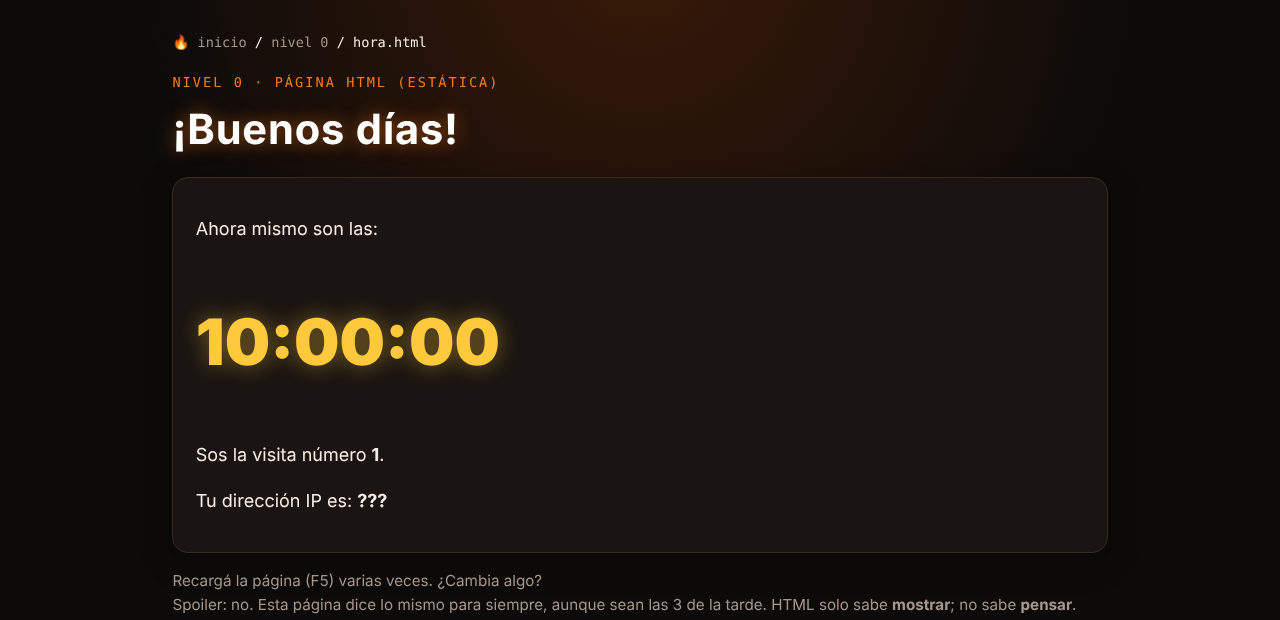
\includegraphics[width=\linewidth]{imagenes/hora-html.png}};\end{minipage}\hfill
\begin{minipage}{0.48\linewidth}\centering{\small\bfseries\color{fuego} hora.php}\\[1mm]\tikz\node[draw=fuego,rounded corners=1mm,inner sep=0pt]{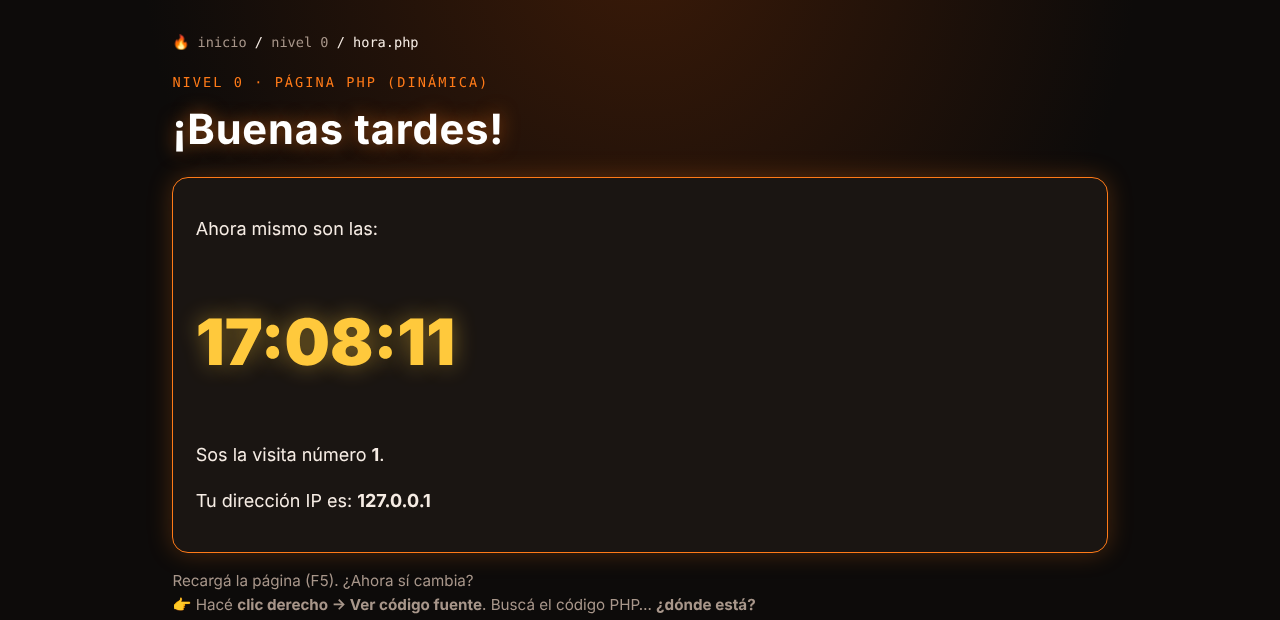
\includegraphics[width=\linewidth]{imagenes/hora-php.png}};\end{minipage}
\end{center}
La página HTML dice \textbf{10:00:00} y «visita número 1» para siempre. La PHP cambia la hora, cuenta tus visitas,
te saluda según el momento del día y sabe tu dirección IP.

\parte{El experimento clave: ver el código fuente}
En \texttt{hora.php}, hacé \textbf{clic derecho $\rightarrow$ Ver código fuente} (o \texttt{Ctrl+U}). Buscá el código PHP\ldots\ \textbf{no está}.
\begin{salida}[lo que recibe el navegador (resumido)]
<h1>¡Buenas tardes!</h1>
<p class="enorme">17:08:11</p>
<p>Sos la visita número <b>3</b>.</p>
\end{salida}
El navegador solo recibió \textbf{el resultado}. El código se ejecutó en el servidor, adentro del contenedor \texttt{fogon-web}.

\parte{El código explicado}
\begin{php}{www/00-gancho/hora.php (la parte PHP)}
<?php
session_start();

$hora = (int) date('H');

if ($hora < 12) {
    $saludo = '¡Buenos días!';
} elseif ($hora < 19) {
    $saludo = '¡Buenas tardes!';
} else {
    $saludo = '¡Buenas noches!';
}

$_SESSION['visitas'] = ($_SESSION['visitas'] ?? 0) + 1;
$ip = $_SERVER['REMOTE_ADDR'];
?>
<h1><?php echo $saludo; ?></h1>
\end{php}
\begin{lineas-explicadas}
1 & \texttt{<?php} abre la «zona PHP». Todo lo que sigue es código que ejecuta el servidor. \\
2 & \texttt{session\_start()} le da a PHP una «memoria» por visitante: así puede contar tus visitas. \\
4 & \texttt{date('H')} pregunta la hora actual (de 0 a 23) y la guarda en la variable \texttt{\$hora}. \\
6--12 & \texttt{if / elseif / else}: según la hora, elige un saludo distinto. (Lo vemos en el nivel 2.) \\
14 & Suma 1 a tus visitas. El \texttt{?? 0} significa «si todavía no había visitas, empezá en 0». \\
15 & \texttt{\$\_SERVER['REMOTE\_ADDR']} es la dirección IP de quien visita la página. \\
16 & \texttt{?>} cierra la zona PHP. Lo que sigue es HTML normal. \\
17 & \texttt{echo} escribe el saludo \textbf{dentro} del HTML. \\
\end{lineas-explicadas}

\begin{comprueba}
\begin{enumerate}
  \item ¿Por qué al ver el código fuente de \texttt{hora.php} no aparece el código PHP?
  \item Si mirás \texttt{hora.php} a las 20:30, ¿qué saludo sale?
  \item ¿Puede alguien que visita tu página leer la contraseña de tu base de datos escrita en un archivo PHP? ¿Por qué?
\end{enumerate}
\end{comprueba}

% =====================================================================
\nivelportada{1}{Hablar: echo y variables}{cianneon}{PHP escribe HTML por vos. Primero, a hablar.}{25 min}{100}

\begin{analogia}
Una \textbf{variable} es una \textbf{cajita con una etiqueta}. En la etiqueta escribís un nombre (\texttt{\$nombre}) y adentro
guardás algo (\texttt{'Ana'}). Cuando necesitás el dato, pedís la cajita por su nombre.
\texttt{echo} es la \textbf{boca} de PHP: lo que le das, lo escribe en la página.
\end{analogia}

\parte{Míralo funcionar}
Abrí en el navegador \texttt{http://localhost:8090/01-hablar/1-echo.php}\\ y, al mismo tiempo, el archivo \texttt{www/01-hablar/1-echo.php} en VS Code.
\captura[0.8\linewidth]{imagenes/echo.png}

\parte{El código explicado}
\begin{php}{www/01-hablar/1-echo.php (resumido)}
<?php
$nombre  = 'Juan Pablo';
$materia = 'Tecnología Web I';
$anio    = 2026;
$precio  = 12.50;
?>
<p>Hola, soy <?php echo $nombre; ?>.</p>
<p><?php echo 'Estudio ' . $materia . ' en el año ' . $anio; ?></p>
<p><?php echo "El cafecito cuesta $precio bolivianos."; ?></p>
<p><?php echo 'Con comillas simples sale: $precio'; ?></p>
<p>Tres cafecitos: <?php echo $precio * 3; ?> Bs.</p>
<p><?= strtoupper($nombre) ?></p>
\end{php}
\begin{lineas-explicadas}
2--5 & Cuatro variables. Todas empiezan con \texttt{\$}. Los \textbf{textos} van entre comillas; los \textbf{números}, sin comillas. Cada línea termina con \texttt{;}. \\
7 & \texttt{echo \$nombre;} escribe el contenido de la cajita \texttt{\$nombre} dentro del párrafo. \\
8 & El \textbf{punto} (\texttt{.}) \textbf{pega} textos: «Estudio » + «Tecnología Web I» + « en el año » + 2026. \\
9 & Con comillas \textbf{dobles}, PHP busca variables adentro y las \textbf{reemplaza} por su valor. \\
10 & Con comillas \textbf{simples}, PHP \textbf{no} reemplaza: sale el texto \texttt{\$precio} tal cual. \\
11 & PHP hace cuentas: \texttt{*} multiplica, \texttt{+} suma, \texttt{-} resta, \texttt{/} divide. \\
12 & \texttt{<?= ... ?>} es un \textbf{atajo} de \texttt{<?php echo ... ?>}. \texttt{strtoupper} pasa a mayúsculas: PHP trae miles de funciones así. \\
\end{lineas-explicadas}

\begin{salida}
Hola, soy Juan Pablo.
Estudio Tecnología Web I en el año 2026
El cafecito cuesta 12.5 bolivianos.
Con comillas simples sale: $precio
Tres cafecitos: 37.5 Bs.
JUAN PABLO
\end{salida}

\begin{modifica}
\begin{enumerate}
  \item Cambiá \texttt{\$nombre} por tu nombre. Guardá (\texttt{Ctrl+S}) y recargá (\texttt{F5}). \xp{10}
  \item Cambiá el precio a \texttt{15}. ¿Qué pasa con el total de tres cafecitos? \xp{10}
  \item Agregá \texttt{\$ciudad = 'Tarija';} y mostrala en un párrafo nuevo con comillas dobles. \xp{10}
  \item Probá \texttt{strtolower} y \texttt{strlen(\$nombre)}. ¿Qué hace cada una? \xp{10}
\end{enumerate}
\end{modifica}

\parte{El reto: tu tarjeta de presentación viva}
Abrí \texttt{www/01-hablar/2-tarjeta.php}. PHP ya calcula tu edad y los días que faltan para la defensa del proyecto:
\begin{php}{lo que PHP calcula solo}
$anioActual = (int) date('Y');
$edad       = $anioActual - $anioNacimiento;

$defensa = strtotime('2026-11-25');
$dias    = (int) ceil(($defensa - time()) / 86400);
\end{php}
\begin{lineas-explicadas}
1 & \texttt{date('Y')} da el año actual. El \texttt{(int)} lo convierte en número entero. \\
2 & Una resta: tu edad (aproximada) sale sola cada año. \\
4 & \texttt{strtotime} convierte una fecha en \textbf{segundos} (así mide PHP el tiempo). \\
5 & Fecha de la defensa menos ahora (\texttt{time()}) $=$ segundos que faltan. Dividido \texttt{86400} (los segundos de un día) $=$ días. \texttt{ceil} redondea hacia arriba. \\
\end{lineas-explicadas}

\begin{reto}[Reto · tu tarjeta \xp{60}]
\begin{enumerate}
  \item \textbf{TODO 1:} poné tus datos reales (nombre, carrera, año de nacimiento, frase).
  \item \textbf{TODO 2:} creá una variable \texttt{\$color} con un color en inglés (\texttt{'orange'}, \texttt{'deepskyblue'}, \texttt{'lime'}\ldots).
  \item \textbf{TODO 3:} usala en el borde de la tarjeta: cambiá \texttt{border-color: orange} por \texttt{border-color: <?= \$color ?>}.
  \item \textbf{Bonus:} si faltan 1 o menos días, que diga «¡Es mañana!». (Vas a necesitar un \texttt{if}: espiá el nivel 2.)
\end{enumerate}
Solución: \texttt{http://localhost:8090/soluciones/2-tarjeta-solucion.php}
\end{reto}

\begin{errores}
\textbf{Pantalla con «Parse error»}: casi siempre falta un \texttt{;} al final de la línea \emph{anterior} a la que dice PHP.\\[1mm]
\textbf{Sale \texttt{\$nombre} escrito tal cual}: usaste comillas simples. Cambiá a dobles o usá el punto.\\[1mm]
\textbf{«Undefined variable»}: escribiste mal el nombre. \texttt{\$Nombre} y \texttt{\$nombre} son \textbf{distintas}.
\end{errores}

\begin{comprueba}
\begin{enumerate}
  \item ¿Con qué símbolo empiezan todas las variables en PHP?
  \item ¿Qué muestra \texttt{echo 'Total: \$precio';}? ¿Y \texttt{echo "Total: \$precio";}?
  \item ¿Para qué sirve el punto (\texttt{.}) en \texttt{'Hola, ' . \$nombre}?
  \item ¿Qué es \texttt{<?= \$x ?>}?
\end{enumerate}
\end{comprueba}

% =====================================================================
\nivelportada{2}{Decidir y repetir: if, arrays y foreach}{fuego}{El código toma decisiones… y hace el trabajo repetitivo por vos.}{30 min}{150}

\begin{analogia}
\textbf{if} es el \textbf{portero} de un boliche: mira tu edad y decide si pasás. Un \textbf{array} es una \textbf{lista}
(como la lista de compras) o una \textbf{ficha} (nombre: Saice, precio: 38). \textbf{foreach} es el \textbf{mozo que recorre todas las
mesas}: hace lo mismo con cada una, sin que tengas que escribirlo diez veces.
\end{analogia}

\parte{Parte A · Decidir con if}
Abrí \texttt{www/02-decidir/1-edad.php}:
\begin{php}{www/02-decidir/1-edad.php (resumido)}
$edad = 17;

if ($edad < 13) {
    $mensaje = 'Sos un niño: menú infantil';
} elseif ($edad < 18) {
    $mensaje = 'Sos adolescente: nada de bebidas para adultos';
} elseif ($edad < 60) {
    $mensaje = 'Sos adulto: acceso completo';
} else {
    $mensaje = 'Adulto mayor: 20 % de descuento';
}
\end{php}
\begin{lineas-explicadas}
3 & \texttt{if (condición) \{ ... \}}: si la condición es verdadera, se ejecuta lo que está entre llaves. \\
5 & \texttt{elseif}: «si no se cumplió lo anterior, probá esto». Se pueden poner varios. \\
9 & \texttt{else}: «en cualquier otro caso». No lleva condición. \\
-- & \textbf{Clave}: PHP prueba de arriba hacia abajo y se queda con la \textbf{primera} condición verdadera. Las demás se ignoran. \\
\end{lineas-explicadas}

\begin{marco}[fuego]{Para comparar}
\renewcommand{\arraystretch}{1.2}
\begin{tabularx}{\linewidth}{>{\ttfamily\bfseries}l X >{\ttfamily\bfseries}l X}
<  & menor & ==  & igual (¡dos signos!) \\
>  & mayor & !=  & distinto \\
<= & menor o igual & \&\& & «y»: las dos condiciones \\
>= & mayor o igual & || & «o»: alcanza con una \\
\end{tabularx}
\end{marco}

\begin{modifica}
\begin{enumerate}
  \item Probá con \texttt{\$edad} igual a 10, 17, 18, 25 y 70. \xp{10}
  \item \textbf{Misión}: agregá el caso «exactamente 18» con el mensaje «¡Felices 18! El postre va por la casa». ¿Dónde tiene que ir para que funcione? \xp{20}
\end{enumerate}
\end{modifica}

\parte{Parte B · Repetir con arrays y foreach}
Abrí \texttt{www/02-decidir/2-menu.php}:
\captura[0.8\linewidth]{imagenes/menu.png}
\begin{php}{www/02-decidir/2-menu.php (resumido)}
$menu = [
    ['plato' => 'Salteña de carne', 'precio' => 10, 'picante' => true],
    ['plato' => 'Saice tarijeño',   'precio' => 38, 'picante' => true],
    ['plato' => 'Tojorí',           'precio' => 12, 'picante' => false],
];
?>
<table>
  <?php foreach ($menu as $item): ?>
    <tr>
      <td><?= $item['plato'] ?></td>
      <td><?= $item['precio'] ?> Bs</td>
    </tr>
  <?php endforeach; ?>
</table>
<p>Hay <?= count($menu) ?> platos.</p>
\end{php}
\begin{lineas-explicadas}
1--5 & Un array de \textbf{fichas}. Cada ficha tiene «casilleros» con nombre: \texttt{'plato'}, \texttt{'precio'}, \texttt{'picante'}. \\
8 & \texttt{foreach (\$menu as \$item)}: «para cada plato del menú, llamalo \texttt{\$item} y hacé lo que sigue». \\
9--12 & \textbf{Una sola fila} de tabla escrita\ldots\ que se repite una vez por cada plato. \\
10 & \texttt{\$item['plato']} saca el casillero \texttt{'plato'} de la ficha actual. \\
13 & \texttt{endforeach;} cierra la repetición. \\
15 & \texttt{count(\$menu)} cuenta cuántos elementos tiene el array. \\
\end{lineas-explicadas}

\begin{marco}[orojp]{El momento mágico}
Agregá un plato nuevo al array, guardá y recargá: \textbf{aparece solo en la tabla}. No tocaste el HTML.
Con 3 líneas de PHP podés generar 3 filas\ldots\ o 3000.
\end{marco}

\parte{El reto: el menú del día}
\begin{reto}[Reto · ¿me alcanza? \xp{80}]
Abrí \texttt{www/02-decidir/3-reto-menu.php}:
\begin{enumerate}
  \item \textbf{TODO 1:} agregá 3 platos al array.
  \item \textbf{TODO 2:} cambiá el \texttt{\$presupuesto}.
  \item \textbf{TODO 3:} en la columna «¿Me alcanza?», con un \texttt{if}: si el precio es menor o igual al presupuesto, mostrá «Sí»; si no, «No».
  \item \textbf{Bonus:} mostrá cuántos platos te alcanzan.
\end{enumerate}
\textbf{Pista del bonus:} creá \texttt{\$alcanzan = 0;} \emph{antes} del \texttt{foreach} y, dentro del \texttt{if}, sumale uno con \texttt{\$alcanzan++;}.
Solución: \texttt{soluciones/3-reto-menu-solucion.php}
\end{reto}

\begin{errores}
\textbf{Usaste \texttt{=} en vez de \texttt{==}}: \texttt{if (\$edad = 18)} no compara, \textbf{asigna}. Siempre da verdadero. Para comparar: \texttt{==}.\\[1mm]
\textbf{El caso de los 18 nunca aparece}: lo pusiste después de \texttt{elseif (\$edad < 60)}, que ya es verdadero para 18. El orden importa.\\[1mm]
\textbf{«Undefined array key»}: escribiste mal el nombre del casillero: \texttt{\$item['Plato']} no es lo mismo que \texttt{\$item['plato']}.
\end{errores}

\begin{comprueba}
\begin{enumerate}
  \item Si \texttt{\$edad = 15}, ¿qué condición se cumple primero en el ejemplo del portero?
  \item ¿Qué diferencia hay entre \texttt{=} y \texttt{==}?
  \item ¿Qué hace \texttt{foreach}? ¿Por qué en el HTML hay una sola fila \texttt{<tr>}?
  \item ¿Cómo sacás el precio de una ficha \texttt{\$item}?
\end{enumerate}
\end{comprueba}

% =====================================================================
\nivelportada{3}{Escuchar: formularios con GET y POST}{verdeneon}{La página te pregunta algo… y PHP escucha la respuesta.}{20 min}{150}

\begin{analogia}
Un formulario es como \textbf{dejarle una nota al cocinero}. Con \textbf{GET}, la nota va \textbf{pegada en la puerta}: cualquiera
que pase la lee (va en la URL). Con \textbf{POST}, la nota va \textbf{dentro de un sobre}: no se ve desde afuera (va en el cuerpo
de la petición). En los dos casos, el cocinero (PHP) la lee y responde.
\end{analogia}

\parte{Míralo funcionar: el Oráculo}
Abrí \texttt{http://localhost:8090/03-escuchar/1-oraculo.php}, poné tu nombre y una pregunta de sí o no.
\captura[0.8\linewidth]{imagenes/oraculo.png}
Ahora \textbf{mirá la barra de direcciones}: \texttt{1-oraculo.php?nombre=Ana\&pregunta=\ldots}. Tus datos viajaron en la URL. Eso es \textbf{GET}.

\parte{El código explicado}
\begin{php}{www/03-escuchar/1-oraculo.php (resumido)}
$respuestas = ['Sí, sin ninguna duda.', 'Las estrellas dicen que NO.', 'Es muy probable.'];

$nombre   = $_GET['nombre']   ?? '';
$pregunta = $_GET['pregunta'] ?? '';

$respuesta = '';
if ($nombre !== '' && $pregunta !== '') {
    $respuesta = $respuestas[array_rand($respuestas)];
}

function e($texto) { return htmlspecialchars($texto, ENT_QUOTES, 'UTF-8'); }
?>
<form method="get">
  <input name="nombre"   value="<?= e($nombre) ?>">
  <input name="pregunta" value="<?= e($pregunta) ?>">
  <button>Consultar al Oráculo</button>
</form>
\end{php}
\begin{lineas-explicadas}
1 & Un array con las respuestas posibles. \\
3--4 & \texttt{\$\_GET} es un array que PHP \textbf{llena solo} con lo que vino en la URL. \texttt{\$\_GET['nombre']} es lo que escribiste en el campo \texttt{name="nombre"}. El \texttt{?? ''} significa «si no vino nada, usá un texto vacío». \\
7 & \texttt{!==} es «distinto». \texttt{\&\&} es «y»: solo responde si escribiste nombre \textbf{y} pregunta. \\
8 & \texttt{array\_rand} elige una posición al azar del array: el Oráculo «adivina». \\
11 & La función \texttt{e()} usa \texttt{htmlspecialchars}: un \textbf{escudo} para mostrar texto que escribió un usuario. Usalo siempre (al final de la clase vas a ver por qué). \\
13 & \texttt{method="get"}: los datos viajan en la URL. \\
14--15 & El atributo \texttt{name} es la \textbf{etiqueta} con la que PHP encuentra cada dato. \\
\end{lineas-explicadas}

\parte{GET vs POST: la contraseña en la URL}
Abrí \texttt{2-login-get.php} y escribí la contraseña \texttt{forja2026}. Funciona\ldots\ pero mirá la URL:
\begin{salida}[la barra de direcciones]
http://localhost:8090/03-escuchar/2-login-get.php?clave=forja2026
\end{salida}
\textbf{Tu contraseña quedó escrita en la URL}: en el historial del navegador, en los registros del servidor y a la vista de
quien mire tu pantalla. Ahora probá \texttt{3-login-post.php}: la URL queda limpia.
\begin{php}{www/03-escuchar/3-login-post.php (lo importante)}
$enviado = ($_SERVER['REQUEST_METHOD'] === 'POST');
$clave   = $_POST['clave'] ?? '';
\end{php}
\begin{lineas-explicadas}
1 & ¿Llegó el formulario? \texttt{REQUEST\_METHOD} dice si la página se pidió con GET (abrirla) o con POST (enviar el formulario). \\
2 & \texttt{\$\_POST} funciona igual que \texttt{\$\_GET}, pero con los datos que vinieron «en el sobre». \\
\end{lineas-explicadas}

\renewcommand{\arraystretch}{1.3}
\begin{tabularx}{\linewidth}{>{\bfseries}p{3.2cm} X X}
\toprule
 & \textbf{GET} & \textbf{POST} \\
\midrule
Dónde viajan los datos & En la URL (\texttt{?clave=...}) & En el cuerpo de la petición \\
Se ven en la barra & Sí & No \\
Se pueden guardar en favoritos & Sí & No \\
Usalo para & Búsquedas, filtros, enlaces & Contraseñas, formularios que guardan datos \\
En PHP & \texttt{\$\_GET['campo']} & \texttt{\$\_POST['campo']} \\
\bottomrule
\end{tabularx}

\begin{ojo}[Importante]
POST \textbf{no cifra} nada: solo esconde los datos de la URL. Con F12 $\rightarrow$ Red se ven igual. Lo que protege una contraseña
en el camino es \textbf{HTTPS} (el candado).
\end{ojo}

\begin{modifica}
\begin{enumerate}
  \item Agregá 3 respuestas nuevas al Oráculo. \xp{20}
  \item Cambiá el Oráculo a \texttt{method="post"} y los dos \texttt{\$\_GET} por \texttt{\$\_POST}. ¿Qué cambia en la URL? \xp{30}
  \item Escribí directamente en la barra: \texttt{1-oraculo.php?nombre=Profe\&pregunta=Hola}. ¿Qué pasa? \xp{20}
\end{enumerate}
\end{modifica}

\begin{errores}
\textbf{«Undefined array key»} al abrir la página: usaste \texttt{\$\_GET['nombre']} sin el \texttt{?? ''}. La primera vez no viene nada.\\[1mm]
\textbf{PHP no recibe el dato}: el \texttt{name} del \texttt{input} no coincide con lo que buscás en \texttt{\$\_GET} o \texttt{\$\_POST}.\\[1mm]
\textbf{Cambiaste a POST y no anda}: tenés que cambiar \textbf{las dos cosas}, el \texttt{method} del formulario y \texttt{\$\_GET} por \texttt{\$\_POST}.
\end{errores}

\begin{comprueba}
\begin{enumerate}
  \item ¿Qué es \texttt{\$\_GET}? ¿Quién lo llena?
  \item ¿Qué relación hay entre \texttt{name="pregunta"} y \texttt{\$\_GET['pregunta']}?
  \item ¿Por qué un login no debe usar GET?
  \item ¿POST cifra la contraseña? ¿Qué la protege de verdad?
\end{enumerate}
\end{comprueba}

% =====================================================================
\nivelportada{4}{Recordar: PHP + MySQL}{lilaneon}{Hasta ahora, cada vez que recargabas, PHP se olvidaba de todo. Ahora abrimos la despensa.}{40 min}{200}

\begin{analogia}
\textbf{MySQL} es la \textbf{despensa} del restaurante: ahí se guardan los ingredientes (los datos) aunque se apague la cocina.
\textbf{PDO} es la \textbf{llave} de la despensa: PHP la usa para entrar, sacar ingredientes (\texttt{SELECT}) y guardar nuevos (\texttt{INSERT}).
\end{analogia}

\parte{La despensa: la base de datos «fogon»}
Ya viene cargada con tres tablas (desde \texttt{db/init.sql}). Para verlas, abrí \texttt{http://localhost:8091} (\textbf{phpMyAdmin}).

\noindent\renewcommand{\arraystretch}{1.25}
\begin{tabularx}{\linewidth}{>{\ttfamily\bfseries}l X}
\toprule
\normalfont\bfseries Tabla & \textbf{Qué guarda} \\
\midrule
menu & 13 platos: \texttt{id}, \texttt{plato}, \texttt{categoria}, \texttt{precio}, \texttt{picante} \\
visitas & El libro de visitas: \texttt{id}, \texttt{nombre}, \texttt{mensaje}, \texttt{creado} \\
contactos & Para el jefe final: \texttt{id}, \texttt{nombre}, \texttt{correo}, \texttt{mensaje}, \texttt{creado} \\
\bottomrule
\end{tabularx}

\parte{La llave: conexion.php}
\begin{php}{www/04-recordar/conexion.php (resumido)}
$host    = getenv('DB_HOST') ?: 'db';
$base    = 'fogon';
$usuario = 'fogon';
$clave   = 'fogon123';

$pdo = new PDO(
    "mysql:host=$host;dbname=$base;charset=utf8mb4",
    $usuario,
    $clave,
    [PDO::ATTR_ERRMODE => PDO::ERRMODE_EXCEPTION,
     PDO::ATTR_DEFAULT_FETCH_MODE => PDO::FETCH_ASSOC]
);
\end{php}
\begin{lineas-explicadas}
1 & \texttt{db} es el \textbf{nombre del contenedor} de MySQL. Dentro de la red de Docker, los contenedores se encuentran por su nombre. \\
6--7 & \texttt{new PDO(...)} crea la conexión. El texto dice: «MySQL, en el host \texttt{db}, base \texttt{fogon}, con caracteres \texttt{utf8mb4}» (para que las tildes, la ñ y los emoji se guarden bien). \\
8--9 & Usuario y contraseña de MySQL. Como esto es PHP, \textbf{nadie desde el navegador puede verlos}. \\
10 & \texttt{ERRMODE\_EXCEPTION}: si algo falla, que PHP avise en lugar de seguir en silencio. \\
11 & \texttt{FETCH\_ASSOC}: cada fila llega como una \textbf{ficha} (array con nombres), igual que en el nivel 2. \\
\end{lineas-explicadas}
Las demás páginas la usan con una sola línea: \texttt{require 'conexion.php';}. Así la llave se escribe una sola vez.

\parte{Leer: el menú desde la base de datos}
Abrí \texttt{http://localhost:8090/04-recordar/1-menu-db.php}. Tocá las categorías de arriba para filtrar.
\captura[0.78\linewidth]{imagenes/menu-db.png}
\begin{php}{www/04-recordar/1-menu-db.php (lo importante)}
require 'conexion.php';
$categoria = $_GET['cat'] ?? '';

if ($categoria === '') {
    $platos = $pdo->query('SELECT plato, categoria, precio FROM menu')->fetchAll();
} else {
    $consulta = $pdo->prepare('SELECT plato, categoria, precio FROM menu WHERE categoria = ?');
    $consulta->execute([$categoria]);
    $platos = $consulta->fetchAll();
}
foreach ($platos as $p) { /* ... una fila de tabla por plato ... */ }
\end{php}
\begin{lineas-explicadas}
1 & Trae la llave: la variable \texttt{\$pdo}. \\
5 & \texttt{query} manda una consulta SQL. \texttt{fetchAll()} trae \textbf{todas} las filas como un array de fichas. \\
7 & \texttt{prepare}: una consulta \textbf{preparada}. El \texttt{?} es un \textbf{hueco}. \\
8 & \texttt{execute([\$categoria])} pone el dato del usuario en el hueco, \textbf{por separado} del SQL. Así nadie puede «colarse» dentro de la consulta. \\
11 & ¡El \textbf{mismo} \texttt{foreach} del nivel 2! Solo cambió de dónde vienen los datos. \\
\end{lineas-explicadas}

\begin{marco}[lilaneon!70!black]{La magia: cambiar la página sin tocar el código}
En phpMyAdmin: base \texttt{fogon} $\rightarrow$ tabla \texttt{menu} $\rightarrow$ \textbf{Insertar}. Agregá tu plato favorito y volvé al menú.
\textbf{Apareció, y no tocaste ni una línea de PHP.} Así funcionan todos los sitios reales: el código queda igual y los datos cambian.
\end{marco}

\parte{Guardar: el libro de visitas}
Abrí \texttt{http://localhost:8090/04-recordar/2-libro.php} y firmá el libro.
\captura[0.78\linewidth]{imagenes/libro.png}
\begin{php}{www/04-recordar/2-libro.php (la parte que guarda)}
if ($_SERVER['REQUEST_METHOD'] === 'POST') {
    $nombre  = trim($_POST['nombre']  ?? '');
    $mensaje = trim($_POST['mensaje'] ?? '');

    if ($nombre !== '' && $mensaje !== '') {
        $guardar = $pdo->prepare('INSERT INTO visitas (nombre, mensaje) VALUES (?, ?)');
        $guardar->execute([$nombre, $mensaje]);
    }
    header('Location: 2-libro.php');
    exit;
}
$mensajes = $pdo->query('SELECT nombre, mensaje, creado FROM visitas ORDER BY id DESC')->fetchAll();
\end{php}
\begin{lineas-explicadas}
1 & Solo guardamos si llegó el formulario (POST). \\
2--3 & \texttt{trim} borra los espacios del principio y del final. \\
6 & \texttt{INSERT INTO ... VALUES (?, ?)}: una consulta preparada con \textbf{dos huecos}. \\
7 & Los datos del usuario van \textbf{aparte}, en el mismo orden que los huecos. \\
9--10 & \texttt{header('Location: ...')} redirige a la misma página. Así, si apretás F5, \textbf{no se guarda el mensaje dos veces}. Este truco se llama PRG (Post, Redirect, Get). \\
12 & Lee los mensajes, del más nuevo al más viejo (\texttt{ORDER BY id DESC}). \\
\end{lineas-explicadas}

\begin{modifica}
\begin{enumerate}
  \item Firmá el libro y buscá tu mensaje en phpMyAdmin (tabla \texttt{visitas}). \xp{30}
  \item En \texttt{1-menu-db.php}, cambiá la consulta para ordenar por precio, de mayor a menor: \texttt{ORDER BY precio DESC}. \xp{30}
  \item Mostrá solo los platos picantes: \texttt{WHERE picante = 1}. \xp{40}
  \item Apagá la cocina (\texttt{.\textbackslash scripts\textbackslash apagar.ps1}), volvé a encenderla y abrí el libro. ¿Siguen los mensajes? ¿Por qué? \xp{40}
\end{enumerate}
\end{modifica}

\begin{errores}
\textbf{«La despensa está cerrada»}: MySQL no está listo. Mirá \texttt{docker compose ps}: \texttt{fogon-db} tiene que decir \texttt{healthy}.\\[1mm]
\textbf{«Table doesn't exist»}: escribiste mal el nombre de la tabla. Son \texttt{menu}, \texttt{visitas} y \texttt{contactos}.\\[1mm]
\textbf{«Unknown column»}: escribiste mal el nombre de una columna en el SQL.\\[1mm]
\textbf{Las tildes salen raras}: faltó \texttt{charset=utf8mb4} en la conexión.
\end{errores}

\begin{comprueba}
\begin{enumerate}
  \item ¿Por qué en \texttt{conexion.php} el host es \texttt{db} y no \texttt{localhost}?
  \item ¿Qué diferencia hay entre \texttt{query} y \texttt{prepare} + \texttt{execute}?
  \item ¿Qué son los \texttt{?} en una consulta preparada?
  \item ¿Para qué sirve el \texttt{header('Location: ...')} después de guardar?
\end{enumerate}
\end{comprueba}

% =====================================================================
\nivelportada{5}{El museo de los 5 errores}{brasa}{Todos los programadores rompen cosas. Los buenos saben leer lo que PHP les dice.}{15 min}{100}

\begin{analogia}
Un mensaje de error \textbf{no es un reto}: es PHP \textbf{ayudándote}. Te dice \textbf{qué} pasó y \textbf{en qué línea}. Aprender a
leerlo es como aprender a leer el tablero del auto: la luz roja no es el problema, es el aviso.
\end{analogia}

\parte{La visita guiada}
Abrí \texttt{http://localhost:8090/05-errores/}. Cada archivo está \textbf{roto a propósito}. Para cada uno: abrilo en el navegador,
leé el error, encontrá la línea en VS Code y arreglalo. \xp{20} por cada error arreglado.

\captura[0.95\linewidth]{imagenes/error1.png}

\renewcommand{\arraystretch}{1.4}
\begin{longtable}{>{\bfseries\color{brasa}}c >{\bfseries}p{3.0cm} >{\raggedright\arraybackslash}p{6.1cm} >{\raggedright\arraybackslash}p{5.2cm}}
\toprule
\# & Error & Lo que dice PHP & Cómo se arregla \\
\midrule
1 & Falta el \texttt{;} & \texttt{\small Parse error: syntax error, unexpected token "echo" ... on line 6} & Agregar \texttt{;} al final de la línea \textbf{anterior} (la 5). \\
2 & Variable sin \texttt{\$} & \texttt{\small Fatal error: Uncaught Error: Undefined constant "nombre"} & Escribir \texttt{\$nombre}. Sin \texttt{\$}, PHP cree que es otra cosa. \\
3 & Comillas simples & No hay error\ldots\ pero sale \texttt{Hola, \$nombre} literal. & Usar comillas dobles o concatenar con el punto. \\
4 & PHP en un \texttt{.html} & No sale nada. En el código fuente, el PHP está crudo. & Renombrar el archivo a \texttt{.php}. Apache solo le pasa a PHP los \texttt{.php}. \\
5 & Variable mal escrita & \texttt{\small Warning: Undefined variable \$nombr} & Escribir el nombre exacto. Ojo con las mayúsculas. \\
\bottomrule
\end{longtable}

\begin{marco}[brasa]{La regla de oro para leer errores}
\begin{enumerate}
  \item Leé \textbf{el tipo}: \emph{Parse error} (escribiste algo que PHP no entiende), \emph{Fatal error} (algo imposible), \emph{Warning} (algo raro, pero sigue).
  \item Leé \textbf{la línea}: \texttt{on line 6}.
  \item Si la línea parece bien, \textbf{mirá la de arriba}: muchas veces el error empezó ahí.
\end{enumerate}
\end{marco}

\begin{comprueba}
\begin{enumerate}
  \item PHP dice «error en la línea 6», pero la línea 6 está bien. ¿Dónde buscás?
  \item ¿Por qué el error de las comillas simples es el más peligroso de los cinco?
  \item ¿Por qué un archivo \texttt{.html} no ejecuta PHP?
\end{enumerate}
\end{comprueba}

% =====================================================================
\nivelportada{X}{Jefe final: PHP en tu proyecto}{oroneon}{Un formulario de contacto que valida, guarda en MySQL y está blindado. Listo para la defensa del miércoles.}{25 min}{250}

\begin{analogia}
Ya sabés cocinar cada ingrediente por separado. El jefe final es \textbf{servir un plato completo}: un formulario que
\textbf{escucha} (POST), \textbf{decide} (valida con \texttt{if}), \textbf{recuerda} (guarda en MySQL) y \textbf{muestra} (con \texttt{foreach}),
usando el escudo \texttt{htmlspecialchars}.
\end{analogia}

\parte{Míralo funcionar}
Abrí \texttt{http://localhost:8090/06-reto-final/contacto.php} y enviá el formulario \textbf{mal a propósito}: un nombre de una
letra, un correo inventado, un mensaje corto.
\captura[0.78\linewidth]{imagenes/contacto-errores.png}

\parte{El código explicado}
\begin{php}{www/06-reto-final/contacto.php (la lógica)}
$errores = [];
$datos   = ['nombre' => '', 'correo' => '', 'mensaje' => ''];

if ($_SERVER['REQUEST_METHOD'] === 'POST') {
    foreach ($datos as $campo => $valor) {
        $datos[$campo] = trim($_POST[$campo] ?? '');
    }
    if (mb_strlen($datos['nombre']) < 2) {
        $errores[] = 'El nombre debe tener al menos 2 letras.';
    }
    if (!filter_var($datos['correo'], FILTER_VALIDATE_EMAIL)) {
        $errores[] = 'El correo no parece válido.';
    }
    if (count($errores) === 0) {
        $guardar = $pdo->prepare('INSERT INTO contactos (nombre, correo, mensaje) VALUES (?, ?, ?)');
        $guardar->execute([$datos['nombre'], $datos['correo'], $datos['mensaje']]);
        header('Location: contacto.php?enviado=1');
        exit;
    }
}
\end{php}
\begin{lineas-explicadas}
1--2 & Un array para juntar los errores y otro para los datos del formulario. \\
5--7 & Un \texttt{foreach} recibe los tres campos de una vez y les quita los espacios. \\
8--10 & \textbf{Validar}: \texttt{mb\_strlen} cuenta las letras (también la ñ y las tildes). \texttt{\$errores[] = ...} agrega un error a la lista. \\
11--13 & \texttt{filter\_var(..., FILTER\_VALIDATE\_EMAIL)}: PHP revisa si el correo tiene forma de correo. El \texttt{!} significa «no». \\
14 & Solo si \textbf{no hubo errores}, guardamos. \\
15--16 & El mismo \texttt{INSERT} preparado del libro de visitas, ahora con tres huecos. \\
17 & PRG: redirige con \texttt{?enviado=1} para mostrar el mensaje de «¡Gracias!». \\
\end{lineas-explicadas}
\textbf{Regla de oro del jefe final:} \emph{nunca confíes en lo que llega del navegador}. Siempre validá antes de guardar.

\parte{Llevalo a tu proyecto FORJA WEB}
\begin{reto}[Jefe final · PHP en tu proyecto \xp{250}]
\begin{enumerate}
  \item Copiá \texttt{contacto.php} y \texttt{04-recordar/conexion.php} a tu proyecto (ajustá la ruta del \texttt{require}).
  \item Creá la tabla \texttt{contactos} en tu base de datos (el \texttt{CREATE TABLE} está en \texttt{db/init.sql}).
  \item Cambiá los datos de conexión por los de tu base.
  \item Dale tu diseño: tus colores, tu logo, tus textos.
  \item Probalo: enviá datos malos (¿muestra los errores?) y datos buenos (¿aparecen en la tabla?).
  \item \textbf{El miércoles, mostralo en la defensa}: «nuestro sitio guarda los mensajes en MySQL con consultas preparadas».
\end{enumerate}
\end{reto}

% =====================================================================
\clearpage
\renewcommand{\seccionactual}{¿HACKEADO?}
\section*{Un momento\ldots\ ¿hackeado?}
\addcontentsline{toc}{section}{Un momento… ¿hackeado?}

Al final de la clase, el profe firma el libro de visitas con un mensaje muy raro:
\begin{salida}[el mensaje del «hacker»]
<h1 style="color:red">HACKEADO</h1><script>alert('hackeado')</script>
\end{salida}
\captura[0.78\linewidth]{imagenes/libro-hackeado.png}
\textbf{La página de todos cambió.} ¿Por qué? Mirá la línea que muestra los mensajes en \texttt{2-libro.php}:
\begin{php}{www/04-recordar/2-libro.php · la línea culpable}
<?= $m['mensaje'] ?>
\end{php}
PHP imprimió el mensaje \textbf{tal cual}, y el navegador lo leyó como \textbf{HTML y JavaScript}\ldots\ y lo ejecutó.
El Oráculo y el contacto no se dejan, porque usan el escudo \texttt{htmlspecialchars}, que convierte \texttt{<} en \texttt{\&lt;}
y así el navegador lo \textbf{muestra} en lugar de \textbf{ejecutarlo}.

\begin{marco}[brasa]{Mañana: hackeá y blindá}
Esto se llama \textbf{XSS} (\emph{Cross-Site Scripting}), y es uno de los ataques más comunes de la web. Mañana vamos a atacar
nuestras propias páginas con XSS e \textbf{inyección SQL}\ldots\ y a blindarlas. Para la clase: \textbf{no lo arregles todavía}.
\end{marco}
\vspace{2mm}
\textbf{Para limpiar el libro} después de la demostración: \texttt{http://localhost:8090/04-recordar/limpiar-libro.php}.
